% !TEX TS-program = pdflatex
% !TEX encoding = UTF-8 Unicode

% 
% (c) 2008, Eung-Shin Lee
% public domain.
% 
\documentclass[10pt,compress,slidetop,%
			   hyperref={unicode},xcolor={svgnames},% sub-package options
			   t]{beamer}
% 이곳에서는 글씨체의 크기를 10 pt로 하였음, t는 본문 내용이 슬라이드의 위(top)부터 시작
% 
% Beamer 저작권
% Copyright 2004      by Till Tantau  <tantau@users.sourceforge.net>.
%       and 2005-2006 by Jorg Cassens <jorg.cassens@idi.ntnu.no>
%


\mode<presentation> 									% 출력 양식을 프레젠테이션으로
{
%	\usetheme{Frankfurt}      							% 템플릿은 프랑크푸르트로

% 템플릿 종류: Antibes, Bergen, Berkerley, Berlin, Boadilla, Copenhagen, Darmstadt, Dresden, Frankfurt, Goettingen, 
%  Hannover, Ilmenau, JuanLesPins, Luebeck, Madrid, Malmoe, Marburg, Montpellier, PaloAlto, Pittsburgh, Rochester,
%  Singapore, Szeged, Warsaw
% 
%	\usecolortheme[named=olive]{structure}		% 색상 결정
 	\usefonttheme[onlymath]{serif}					% 수학공식에서 사용하는 글씨체 
  % \useoutertheme{infolines}
  % or whatever

  \setbeamercovered{transparent}						% overlay 사용 
  % or whatever (possibly just delete it)
}

%==================  필요한 패키지 설정 ===============
\usepackage{verbatim}
\usepackage{pdfpages}
\usepackage{multimedia}
\usepackage{animate}
\usepackage{booktabs}

% 
\usepackage{bm}% bold math
\usepackage{amsmath,amssymb,amscd}
\usepackage{subeqnarray}
\usepackage{mathptmx}
% 
\usepackage{helvet}
\usepackage{courier}
\usepackage{relsize}
% 
\usepackage{colortbl}
\usepackage{wasysym}
%
\usepackage{tikz}
\usetikzlibrary{arrows,shapes,calc,patterns}
\tikzstyle{every picture}+=[remember picture]
\usetikzlibrary{%
    decorations.pathreplacing,%
    decorations.pathmorphing%
}
% ================== 한글 사용 =====================
\usepackage{dhucs}
\usepackage{ifpdf}
\ifpdf
  \input glyphtounicode\pdfgentounicode=1
\fi
%==============================================
%
%================ dual screen =======================
%\setbeameroption{show notes on second screen=left} 
%\setbeamertemplate{note page}[compress] 
%==============================================
% 
%================ 제목에 사용할 글씨체 설정 ============== 
%\setbeamerfont{title}{shape=\itshape,family=\rmfamily}
%\setbeamerfont{frametitle}{family=\rmfamily}
%\usepackage[T1]{fontenc}
% Or whatever. Note that the encoding and the font should match. If T1
% does not look nice, try deleting the line with the fontenc.
%===============================================
%
%==================  표지 만들기 =====================
\title % (optional, use only with long paper titles)
{세번째: 온실가스-산업연관표}
%\subtitle{\LaTeX 기초강좌 (2008년 가을, 공주대학교)}


\author{강성원 }													% 저자(발표자)

% Till Tantau\author{{1} \and
% J\"{o}rg Cassens\inst{2}

\institute[] 															% (optional, but mostly needed) 소속기관 약자 표기
{KEI}													% 표지에 나타나는 소속기관 full name
% - Use the \inst command only if there are several affiliations.
% - Keep it simple, no one is interested in your street address.

\date[08-11-09] 														% (optional, should be abbreviation of conference name)
{2016.08.05}																			% 날짜 지정: \today
% - Either use conference name or its abbreviation.
% - Not really informative to the audience, more for people (including
%   yourself) who are reading the slides online

\subject{Beamer}
% This is only inserted into the PDF information catalog. Can be left out.

% Delete this, if you do not want the table of contents to pop up at
% the beginning of each subsection:
%===============================================
%
% ====================  차 례 ======================
 \AtBeginSection[]
 {
 \begin{frame}<beamer>
    \frametitle{차 례}
    \tableofcontents[currentsection,hideallsubsections]
    %\tableofcontents[currentsection,currentsubsections]
  \end{frame}
}
%===============================================
%
%
%==========================  본문 시작 ==============================
\begin{document}
% 
%=================  표지를  화면으로 나타나기 =============
\begin{frame}
  \titlepage
\end{frame}
%===============================================
%
% ******************************
\section{Introduction}
%*******************************

%------------------------------- 슬라이드  --------------------------------------------------
\begin{frame}
	\frametitle{기본 개념}
	\begin{enumerate}
	\item{1차 에너지 (TPES: Total Primary Energy Supply)}
		\begin{itemize}
		\item{정의: 자연이 제공한 그대로의 가공하지 않은 에너지.}
		\item{TPES = 국내생산 + 수입-수출-국제 Bunkering + 재고증가 - 재고감소}
		\item{TPES = 최종에너지소비 + 전환손실}
		\end{itemize}
	\item{전환(Transformation)}
		\begin{itemize}
		\item{에너지의 형태를 변화시키는 과정}
		\end{itemize}
	\item{최종 에너지(TFC: Total Final (Energy) consumption)}
      	\begin{itemize}
		\item{유효에너지로 변환되기 위해 소비자에게 제공되는 에너지}
		\item{TFC = 최종에너지 소비자에게 공급된 에너지양으로 전환손실 및 에너지산업체의 자체소비는 제외함 }
		\end{itemize}
	\item{에너지 Balance}
		\begin{itemize}
		\item{플로우(Flow)의 개념으로 일정기간동안 일정지역내 에너
지의 투입과 산출간의 균형을 나타내는 표}
		\item{형태: 에너지원을 가로축, 에너지수급량
을 세로축에 나타내는 행렬(Matrix)방식을 채택}
		\end{itemize}
	\end{enumerate}
	
\end{frame}
%----------------------------------------------------------------------------------------------
%
%-------------------------------- 슬라이드  -------------------------------------------------
\begin{frame}
	\frametitle{에너지 Balance (한국)}
	  	\begin{figure}
	\centering
	 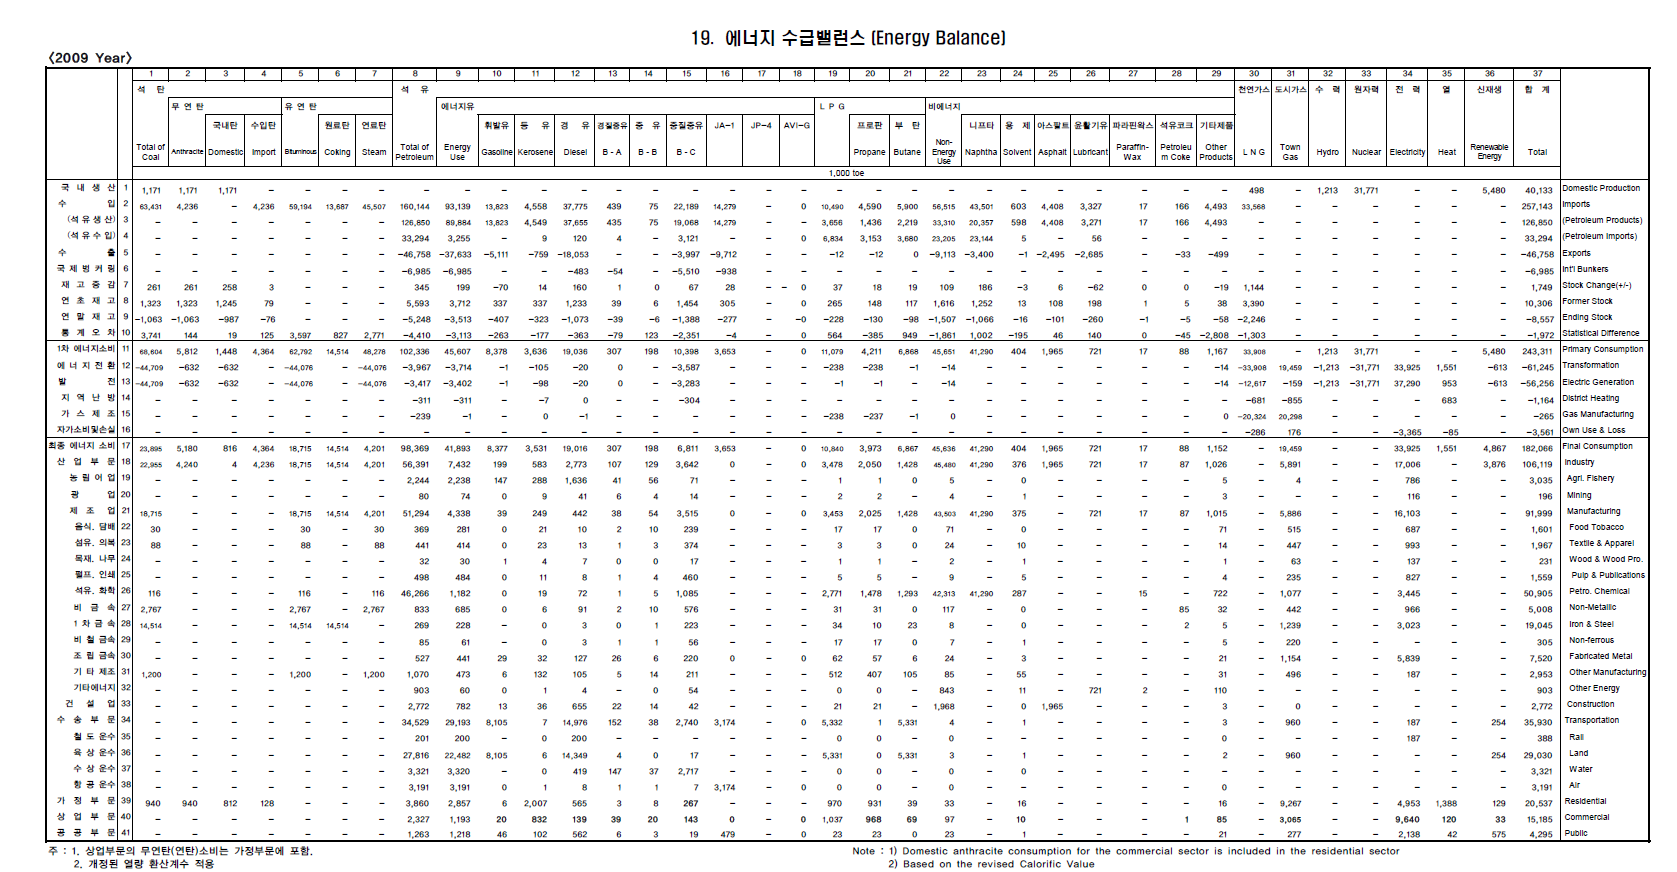
\includegraphics[width=1.00\textwidth]{EBK.png}
	%\caption{}
	\label{IEA world balance}
	\end{figure}	
	
\end{frame}
%----------------------------------------------------------------------------------------------

%
%-------------------------------- 슬라이드  -------------------------------------------------
\begin{frame}
	\frametitle{에너지 Balance (한국-약식)}
	  	\begin{figure}
	\centering
	 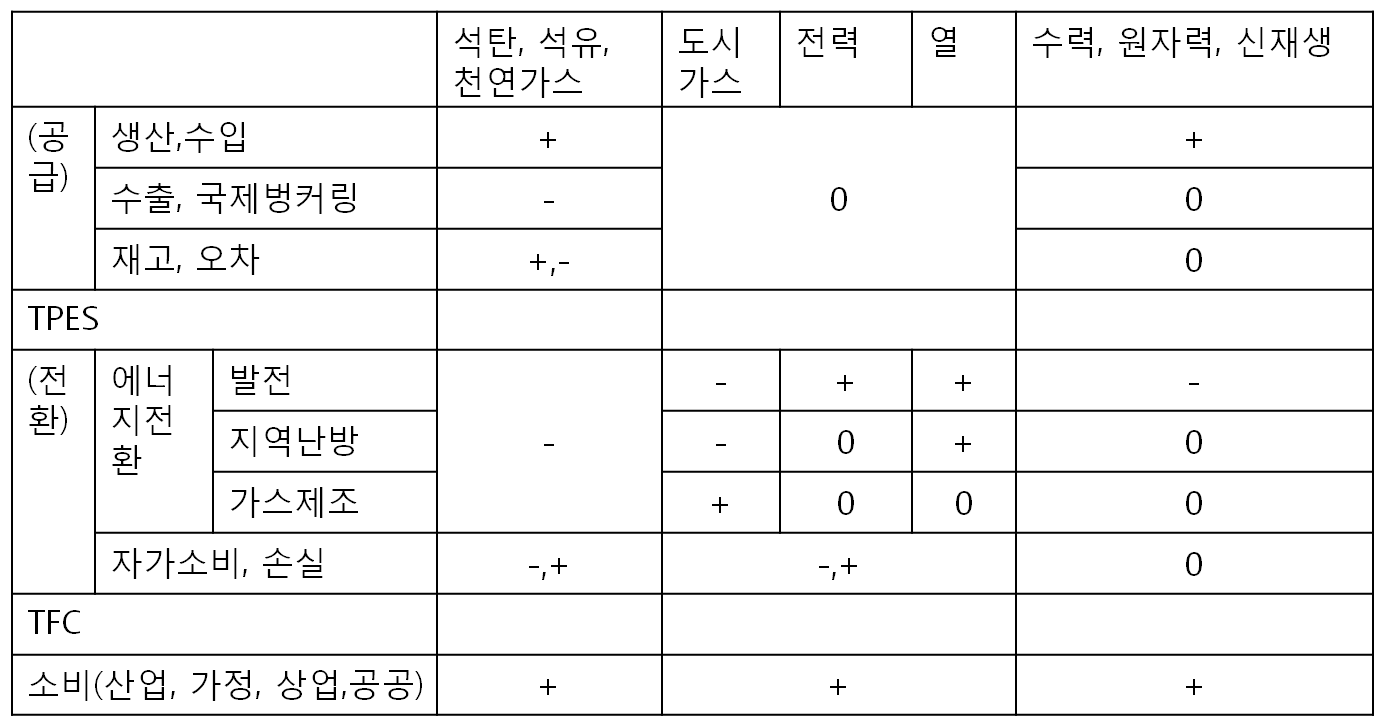
\includegraphics[width=1.00\textwidth]{EBKS.png}
	%\caption{}
	\label{IEA world balance}
	\end{figure}	
	
\end{frame}
%----------------------------------------------------------------------------------------------

%-------------------------------- 슬라이드  -------------------------------------------------
\begin{frame}
	\frametitle{에너지 밸런스와 1차에너지, 최종에너지}
	  	\begin{figure}
	\centering
	 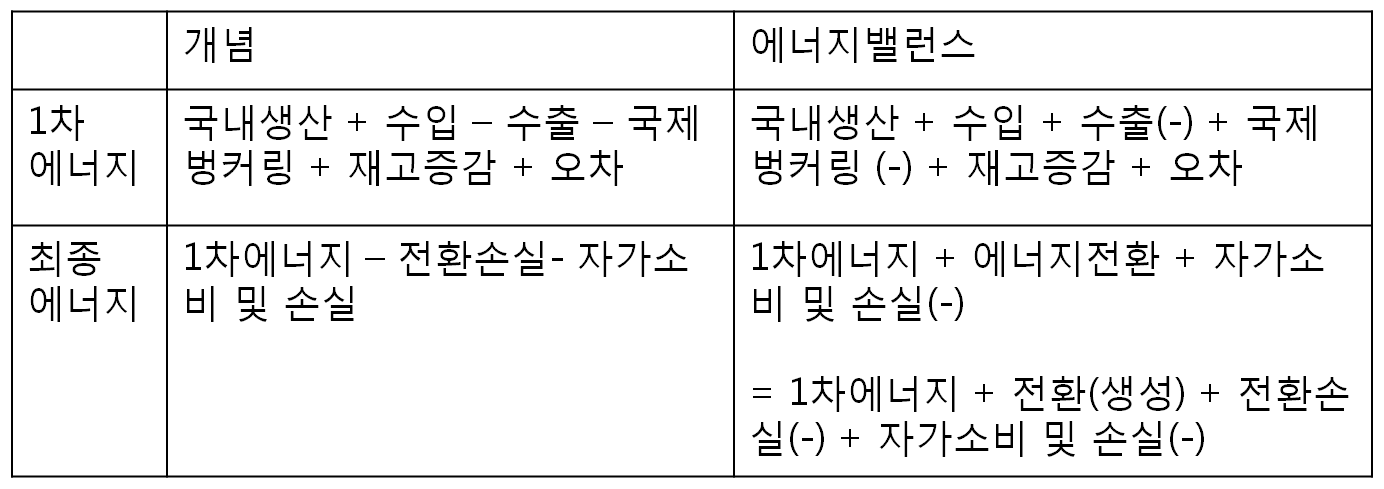
\includegraphics[width=1.00\textwidth]{Definition.png}
	%\caption{}
	\label{IEA world balance}
	\end{figure}	
	
\end{frame}
%----------------------------------------------------------------------------------------------

%-------------------------------- 슬라이드  -------------------------------------------------
\begin{frame}
	\frametitle{산업연관표-에너지 밸런스: TPSE + 전환 E $\Rightarrow$ TFC}
	  	\begin{figure}
	\centering
	 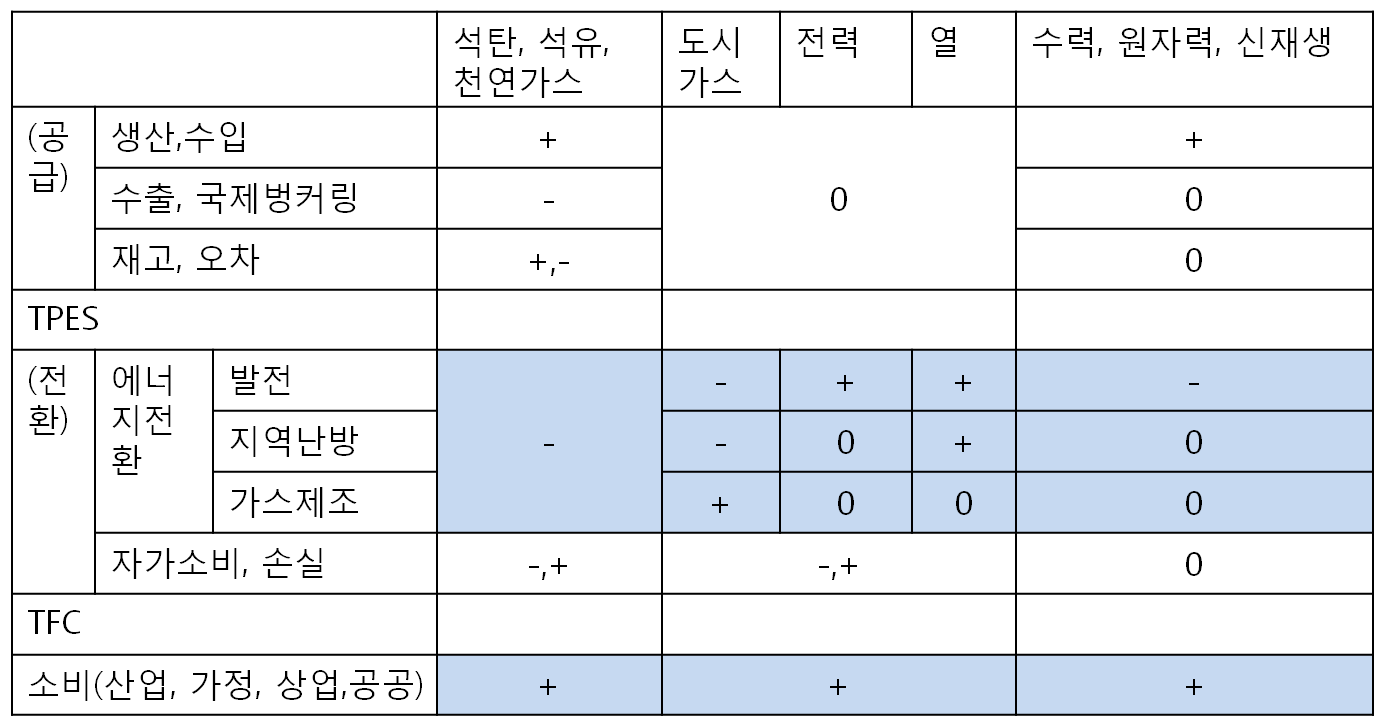
\includegraphics[width=1.00\textwidth]{EBKtarget.png}
	%\caption{}
	\label{IEA world balance}
	\end{figure}	
	
\end{frame}
%----------------------------------------------------------------------------------------------


% 
%*******************************
\section{Process}
%*******************************
%
%------------------------------- 슬라이드  --------------------------------------------------
\begin{frame}
	\frametitle{에너지 IO, 온실가스 IO 생성}
	\begin{itemize}
	\item{Step 1: 순 발열량 에너지 Balance 구축}
	\bigskip
		\begin{itemize}
		\item{ 순 발열량 Balance = 전환계수 $\times$ 총 발열량 Balance}
		\end{itemize}
	\bigskip
	\item{Step 2: 에너지원별 '총수요' 파악 (순 에너지 Balance 사용)}
	\bigskip
		\begin{itemize}
		\item{ 총수요($E_i$)= 1차에너지 소비 혹은 최종에너지소비+전환손실}
		\end{itemize}
	\bigskip
	\item{Step 3: 에너지 '총수요'를 산업연관표에 할당 (에너지 IO 생성)}
         \begin{itemize}
		\item{ 할당($E_{i,(j,f)}$) = 총수요($E_i$) $\times$ $\frac{IO_{i,(j,f)}}{\Sigma_j IO_{i,j}\mbox{(중간재수요)}+\Sigma_f IO_{i,f}\mbox{(최종수요)}}$}
		\end{itemize}
	\bigskip
	\item{Step 4: 온실가스 계산 = 배출계수$\times$할당 에너지 (온실가스 IO 생성)}
		\begin{itemize}
		\item{ 온실가스($G_{ij}$) = 배출계수($\theta_i$)$\times$ 할당 에너지$(E_{ij})$}
		\end{itemize}
	\end{itemize}
	
\end{frame}
%----------------------------------------------------------------------------------------------
%
%*******************************
\section{Step 1: 순 발열량 에너지 Balance 구축}
%*******************************
%
%------------------------------- 슬라이드  --------------------------------------------------
\begin{frame}
	\frametitle{Step 1: 순 발열량 에너지 Balance 구축}
	\begin{enumerate}
	\item{기본 공식 (i : 에너지원)}
	\begin{displaymath}
	\mbox{순 발열량} (E_i) =\mbox{총 발열량} (E^*_i) \times\frac{\mbox{석유환산계수(순발열량기준)}_i}{\mbox{석유환산계수(총발열량기준)}_i}
	\end{displaymath}
		\begin{itemize}
		\item{석유환산계수: 2010에너지통계연보}
		\end{itemize}
	\item{ Wax, Asphalt, Solvent 는 배출량을 산정하지 않아서 순발열량을 0 으로 간주}
    \bigskip
	\item{ 기타제품(석유)은 석유환산계수가 존재하지 않아서 전환계수를 구할 수 없음$\rightarrow$ 0.93953으로 대치}
	\end{enumerate}
	
	%\begin{itemize}
	%\item{input: EB\_G.csv, CF.csv}
	%\item{process: ghg.r (line 40:45)}
	%\item{output:EB\_N}
	%\end{itemize}
	
\end{frame}
%----------------------------------------------------------------------------------------------

%
%*******************************
\section{Step 2: 에너지 원별 총수요 파악}
%*******************************
%
%------------------------------- 슬라이드  --------------------------------------------------
\begin{frame}
	\frametitle{Step 2: 에너지 원별 총수요 파악-(1) 기본공식}
%	\begin{enumerate}
%	\item{기본공식}
\begin{eqnarray*}
\mbox{총수요}&=&\mbox{최종에너지소비}\\
	&-&\{\mbox{발전}\times I(\mbox{발전}\le 0)+\mbox{지역난방}\times I(\mbox{지역난방}\le 0)\\
	& &+\mbox{가스제조}\times I(\mbox{가스제조}\le 0)\\
	& & +\mbox{자가소비 및 손실}\times I(\mbox{자가소비 및 손실}\le 0)\}\\
	&-&(\mbox{수출}+\mbox{국제벙커링}+\mbox{재고증감})\\
=\mbox{최종에너지소비}&-&\mbox{전환손실}-(\mbox{수출}+\mbox{국제벙커링}+\mbox{재고증감})
\end{eqnarray*}
\begin{small}
\begin{displaymath}
=\left\{\begin{array}{lr}
\mbox{1차에너지공급}-(\mbox{수출}+\mbox{국제벙커링}+\mbox{재고증감})&(\mbox{Not 도시가스, 전력, 열})\\
\mbox{전환생성}-(\mbox{수출}+\mbox{국제벙커링}+\mbox{재고증감})&(\mbox{도시가스, 전력, 열})
\end{array}\right.
\end{displaymath}
\end{small}
\smallskip
\begin{small}
수출 및 재고증감 과정에서 발생하는 온실가스는 계상하지 않으므로 수출, 국제벙커링, 재고증감 과정의 에너지 증감도 무시$\rightarrow$ $\mbox{수출}=0, \mbox{국제벙커링} =0,\mbox{재고증감}=0$ 
\end{small}
\begin{displaymath}
\mbox{총수요}=\left\{\begin{array}{ll}
\mbox{1차에너지공급}&(\mbox{for Not 도시가스, 전력, 열})\\
\mbox{전환생성}&(\mbox{for 도시가스, 전력, 열})
\end{array}\right.
\end{displaymath}


%	\end{enumerate}
%\end{\small}	
\end{frame}
%----------------------------------------------------------------------------------------------
%
%-------------------------------- 슬라이드  -------------------------------------------------
\begin{frame}
	\frametitle{에너지 총수요 기본공식}
	  	\begin{figure}
	\centering
	 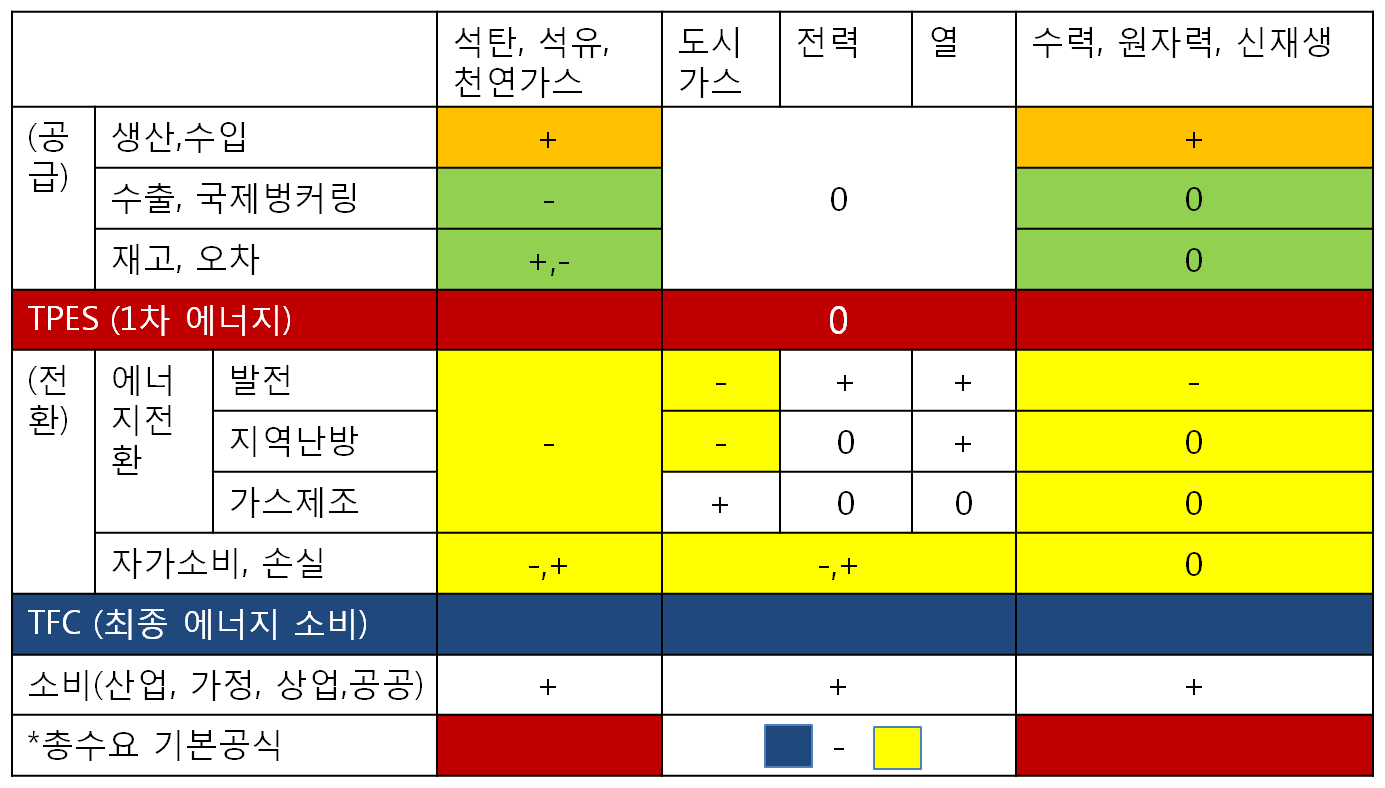
\includegraphics[width=1.00\textwidth]{Edformula.png}
	%\caption{}
	%\label{IEA world balance}
	\end{figure}	

\end{frame}
%----------------------------------------------------------------------------------------------

%-------------------------------- 슬라이드  -------------------------------------------------
\begin{frame}
	\frametitle{Step 2: 에너지 원별 총수요 파악-(1) 기본공식 활용}
\begin{enumerate}
\item{석탄, 석유, 천연가스: 기본공식}
\begin{itemize}
\item{총수요 = 1차에너지}
\end{itemize}
\smallskip

\item{수력, 원자력: 기본공식 $\times$ 보정계수}
\begin{itemize}
\item{총수요 = 1차에너지$\times\frac{860}{2150}$}
\end{itemize}
\smallskip

\item{화력 및 자가발전 전력: 기본공식 - 수력 - 원자력-신재생 발전}
\begin{itemize}
\item{총수요 = $\mbox{전환생성}-\mbox{수력총수요}-\mbox{원자력총수요}-\mbox{신재생 발전}$}
\end{itemize}
\smallskip

\item{도시가스: 천연가스 1차에너지 수요를 사용}
\begin{itemize}
\item{산업연관표: 천연가스가 도시가스 원료로만 사용}
\item{에너지 밸런스: 천연가스가 발전, 지역난방, 가스제조에 사용 }
\begin{itemize}
\item{발전, 지역난방에 투입된 천연가스로부터 발생하는 온실가스를 도시가스 사용 시 발생하는 온실가스에 포함}
\end{itemize}
\end{itemize}

\end{enumerate} 	
%input : EB\_N, process: ghg.r line 80-142	, output:E.Demand\_total	
\end{frame}
%----------------------------------------------------------------------------------------------
% 
%
%------------------------------- 슬라이드  --------------------------------------------------
\begin{frame}
	\frametitle{Step 2: 에너지 원별 총수요 파악-(2) 도시가스}
  	\begin{figure}
	\centering
	 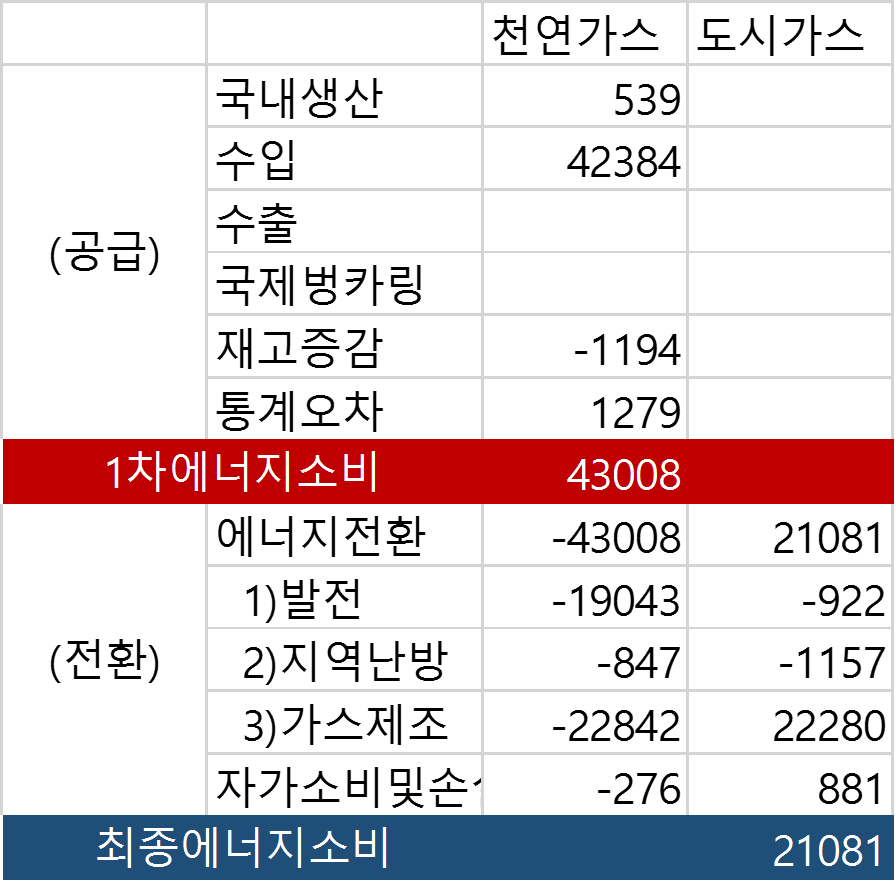
\includegraphics[width=0.5\textwidth]{Citigas.png}
	%\caption{}
	%\label{IEA world balance}
	\end{figure}	

	
\end{frame}
%----------------------------------------------------------------------------------------------

%-------------------------------- 슬라이드  -------------------------------------------------
\begin{frame}
	\frametitle{에너지 총수요: 산업-에너지원 match}
	  	\begin{figure}
	\centering
	 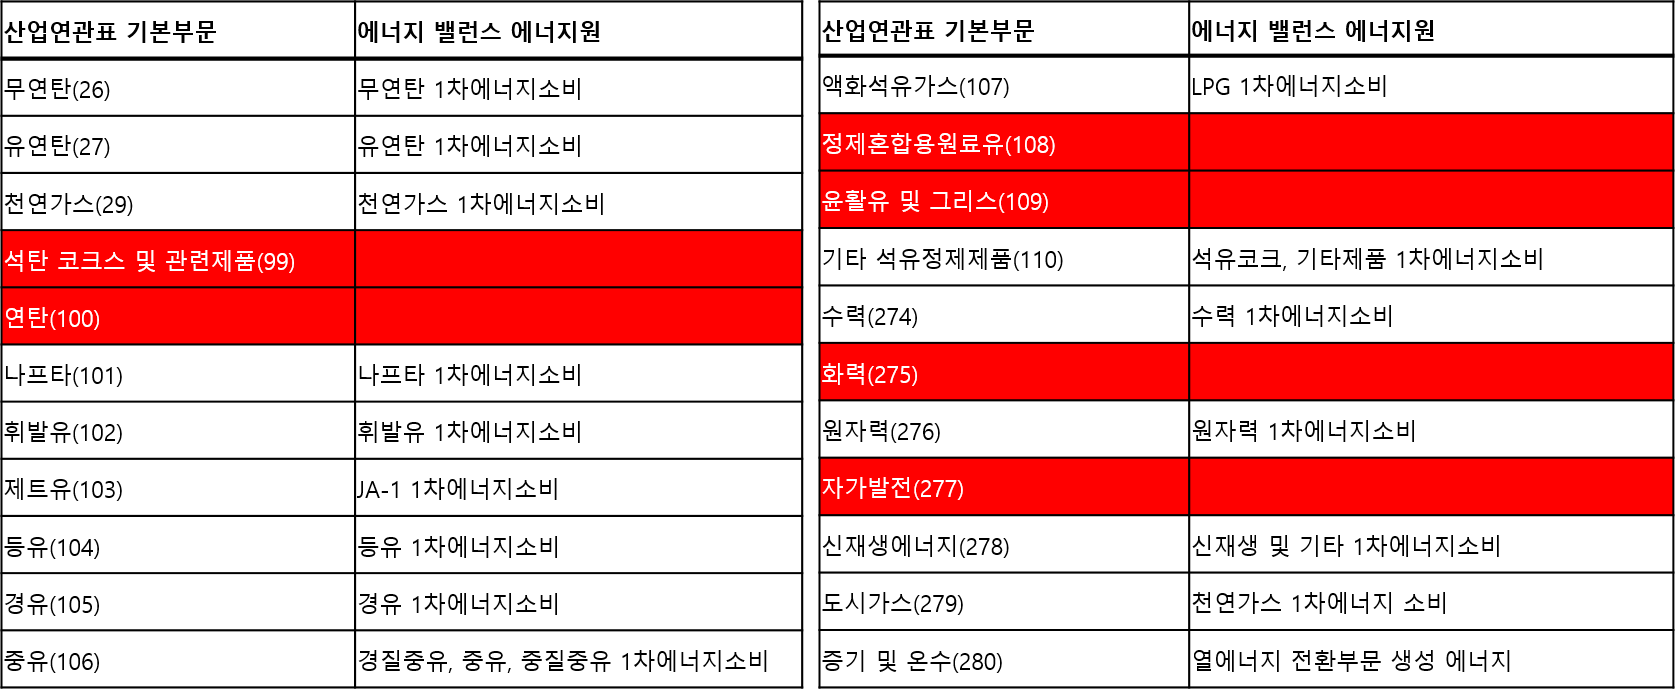
\includegraphics[width=1.00\textwidth]{match.png}
	%\caption{}
	%\label{IEA world balance}
	\end{figure}	
\begin{scriptsize}
%\begin{itemize}
%\item{input : %E.Demand\_total,E.Demand\_Crude,E.Demand\_Coalbriquette,E.Demand.Other\_c,"IO\_whole\_2009.csv"}
%\item{process : ghg.r line 243-294}
%\item{output :E.Demand\_IO }
%\end{itemize}
\end{scriptsize} 	
\end{frame}
%----------------------------------------------------------------------------------------------

%
%------------------------------- 슬라이드  --------------------------------------------------
\begin{frame}
	\frametitle{Step 2: 에너지 원별 총수요 파악: 에너지 Balance에 해당 항목이 부재한 경우}	
	\begin{enumerate}
	\item{연탄: 가정부문 소비 무연탄 }
	\item{석탄코크스및 관련제품: 유연탄 중 발전으로 전환되지 않은 양을 기준으로 재구성 }
	\item{정제혼합용원료유,윤활유 및 그리스: 윤활기유 1차에너지 소비를 산업연관표를 사용하여 분할}
	\item{화력발전, 자가발전: '화력 및 자가발전 총수요'를 산업연관표를 사용하여 분할}
	\end{enumerate}
%\begin{itemize}
%\item{input : EB\_N, "OilData\_2009.csv", "IO\_Domestic\_2009.csv", "IO\_Import\_2009.csv","IO\_whole\_2009.csv"}
%\item{process : ghg.r line 143-242}
%\item{output : E.Demand\_Crude,E.Demand\_Coalbriquette,E.Demand.Other\_c}
%\end{itemize} 		
\end{frame}
%----------------------------------------------------------------------------------------------
%


%------------------------------- 슬라이드  --------------------------------------------------
\begin{frame}
	\frametitle{Step 2: 에너지 원별 총수요 파악-(3-1) 연탄, 기타석탄제품}
	\begin{itemize}
	\item{연탄: 에너지 Balance 상의 무연탄 국내탄 항목은 실제 연탄과는 관계 희박}
		\begin{itemize}
		\item{연탄은 발전용으로 직접 사용되지 않음}
		\item{무연탄 국내탄 최종에너지수요 중 가계수요 에너지를 연탄 에너지 총수요로 사용}	
		\end{itemize}
	\bigskip	
	\item{기타석탄제품: 에너지 Balance 상에는 기타석탄제품이 없지만 IO 에는 존재(코크스)}
	\begin{itemize}		
		\item{기타석탄제품 총수요: 발전에 투입되지 않은 유연탄(유연탄 잔여분) 중 기타석탄제품에 투입된 양 }	
	\end{itemize} 	
\begin{small}
			\begin{eqnarray*}
			& &\mbox{기타석탄제품 총수요}\\ 
			&=&\{\mbox{유연탄 1차에너지수요} -\mbox{유연탄 발전 전환량}\times I(\mbox{유연탄 발전 전환량$>$0})\}\\
			&\times&\frac{\mbox{IO 총거래표 기타석탄제품 투입 유연탄(금액)}}{\mbox{IO 총거래표 유연탄 총수요액-IO 총거래표 발전 투입 유연탄(금액)}} 
			\end{eqnarray*}
			총수요액 = 중간수요액($\Sigma_j IO_{i,j}$) + 가계최종수요액($Household_i$)
\end{small}

	\end{itemize}
	
\end{frame}
%----------------------------------------------------------------------------------------------

%------------------------------- 슬라이드  --------------------------------------------------
\begin{frame}
	\frametitle{Step 2: 에너지 원별 총수요 파악-(3-2) 정제혼합용원료유, 윤활유 및 그리스 }

에너지 Balance 상 윤활기유 1차에너지 소비를 산업연관표를 이용하여 분할 
\begin{footnotesize}
\begin{eqnarray*}
			& &\mbox{1. 정제혼합용원료유}\\ 
			&=&\mbox{윤활기유 1차에너지}\\
			&\times&\frac{\mbox{IO 총거래표 정제혼합용원료유 총수요액 }}{\mbox{IO 총거래표 정제혼합용원료유 총수요액 + IO 총거래표 윤활유 및 그리스 총수요액}} 
			\end{eqnarray*}
			\begin{eqnarray*}
			& &\mbox{2. 윤활유 및 그리스 }\\ 
			&=&\mbox{윤활기유 1차에너지}\\
			&\times&\frac{\mbox{IO 총거래표 윤활유 및 그리 총수요액 }}{\mbox{IO 총거래표 정제혼합용원료유 총수요액 + IO 총거래표 윤활유 및 그리스 총수요액}} 
			\end{eqnarray*}
\end{footnotesize}	
\end{frame}
%----------------------------------------------------------------------------------------------


%------------------------------- 슬라이드  --------------------------------------------------
\begin{frame}
	\frametitle{Step 2: 에너지 원별 총수요 파악-(3-3) 화력발전, 자가발전}

에너지 Balance 상 전력 전환부문 생성에너지에서 에서 수력 1차에너지 수요, 원자력 1차에너지 수요, 신재생 발전수요를 제외한 값을 분할 
\begin{eqnarray*}
			& &\mbox{1. 화력발전 총수요}\\ 
			&=&(\mbox{전력 전환부문 생성 에너지 - 수력 1차에너지 수요}\\
			& &-\mbox{원자력 1차 에너지 수요 -신재생 발전 수요})\\
			&\times&\frac{\mbox{IO 총거래표 화력 총수요액 }}{\mbox{IO 총거래표 화력 총수요액 + IO 총거래표 기타발전 총수요액}} 
			\end{eqnarray*}
			\begin{eqnarray*}
			& &\mbox{2. 자가발전 총수요}\\ 
			&=&(\mbox{전력 전환부문 생성 에너지 - 수력 1차에너지 수요}\\
			& &-\mbox{원자력 1차 에너지 수요 -신재생 발전 수요})\\
			&\times&\frac{\mbox{IO 총거래표 자가발전 총수요액 }}{\mbox{IO 총거래표 화력 총수요액 + IO 총거래표 자가발전 총수요액}} 
			\end{eqnarray*}
	
\end{frame}
%----------------------------------------------------------------------------------------------


%*******************************
\section{Step 3: 에너지 '총수요'를 산업연관표에 할당 }
%*******************************

%------------------------------- 슬라이드  --------------------------------------------------
\begin{frame}
	\frametitle{Step 3: 에너지 '총수요'를 산업연관표에 할당-(1) 기본공식}
\bigskip
산업별 에너지 '총수요'를 산업연관표의 중간수요액/가계수요액을 기준으로 각 산업으로 분할
\smallskip
\begin{small}
\begin{eqnarray*}
			\mbox{에너지 중간수요} (E_{ij})&=&\mbox{에너지 총수요}(E_i)\times\frac{IO_{ij}}{\Sigma_j IO_{ij}+Household_i}\\
			\mbox{에너지 가계수요} (E_{i,h})&=&\mbox{에너지 총수요}(E_i)\times\frac{Household_i}{\Sigma_j IO_{ij}+Household_i}\\
\end{eqnarray*}
\end{small}
%\item{예외 1. Naphta는 석유화학제품(143-171)에 투입된 중간수요액만을 사용하여 할당}
%\begin{eqnarray*}
%			& &\mbox{에너지 중간수요} (E_{ij}|_{143\le j \le 171})\\
%			&=&\mbox{에너지 총수요}(E_i)\times\frac{\mbox{IO 총거래표 중간수요액}_{ij|143\le j \le 171}}{\sum_{143\le j \le 171}%\mbox{IO 총거래표 중간수요액}_{ij}}
%\end{eqnarray*}

%\begin{itemize}
%\item{input : E.Demand\_IO, IO\_whole}
%\item{process : ghg.r line 295-330}
%\item{output :Energy\_BE\_overall }
%\end{itemize} 
		
\end{frame}
%----------------------------------------------------------------------------------------------

%------------------------------- 슬라이드  --------------------------------------------------
\begin{frame}
	\frametitle{Step 3: 에너지 '총수요'를 산업연관표에 할당-(2) 우선할당 }
\bigskip
산업별 에너지 '총수요'의 일부를 산업연관표 중간수요에 직접 할당하고 나머지를 산업연관표 중간수요액 기준으로 분할
\smallskip

\begin{small}
\begin{eqnarray*}
\mbox{에너지 중간수요} (E_{ij|j\in J})&=&\overline{E}_{ij}(\mbox{에너지밸런스 특정항목})\\
\mbox{에너지 중간수요} (E_{ij|j \notin J})&=&(\mbox{에너지 총수요}(E_i)-\sum_{j\in J}E_{ij})\\
& &\times\frac{IO_{ij| j \notin J}}{\Sigma_{j}IO_{ij}+Household_i-\sum_{j\in J}IO_{ij}}\\
\mbox{에너지 가계수요} (E_{i,h})&=&(\mbox{에너지 총수요}(E_i)-\sum_{j\in J}E_{ij})\\
& &\times\frac{Household_h}{\Sigma_{j}IO_{ij}+Household_i-\sum_{j\in J}IO_{ij}}
\end{eqnarray*}
\end{small}


%\begin{itemize}
%\item{input : E.Demand\_IO, IO\_whole}
%\item{process : ghg.r line 331-410}
%\item{output :Energy\_BE\_residual,Energy\_BE  }
%\end{itemize} 
\end{frame}
%----------------------------------------------------------------------------------------------

%-------------------------------- 슬라이드  -------------------------------------------------
\begin{frame}
	\frametitle{에너지 중간수요 우선할당: 무연탄, 유연탄, 중유, 도시가스}
\begin{small}
\begin{table}[htbp]
  \centering
  \caption{에너지 우선 할당}
    \begin{tabular}{ll}\hline\hline
    산업연관표 & 에너지 밸런스 \\\hline
    연탄(100) 투입 무연탄(26) & 가정 소비 무연탄 \\
    화력(275) 투입 무연탄(26) & 전력 전환 유연탄 \\
    화력(275) 투입 유연탄(27) & 전력 전환 무연탄 \\
    화력(275) 투입 중유(106) & 전력 전환 경질중유, 중유, 중질중유 \\
    화력(275) 투입 도시가스(279) & 전력 전환 도시가스, 천연가스 \\
    증기 및 열에너지(280) 투입 도시가스(279) & 열에너지 전환 도시가스, 천연가스 \\\hline
    \end{tabular}%
  \label{tab:addlabel}%
\end{table}%
\end{small}
\begin{itemize}
\item{에너지밸런스에는 천연가스가 발전/지역난방에 사용되지만 산업연관표에서는 천연가스가 전량 도시가스 생산에만 투입됨.} 
\item{발전/지역난방에 사용되는 천연가스 에너지를 도시가스 에너지에 포함}
\end{itemize}
	
\end{frame}
%----------------------------------------------------------------------------------------------


%-------------------------------- 슬라이드  -------------------------------------------------
\begin{frame}
	\frametitle{에너지 중간수요 직접할당}
	  	\begin{figure}
	\centering
	 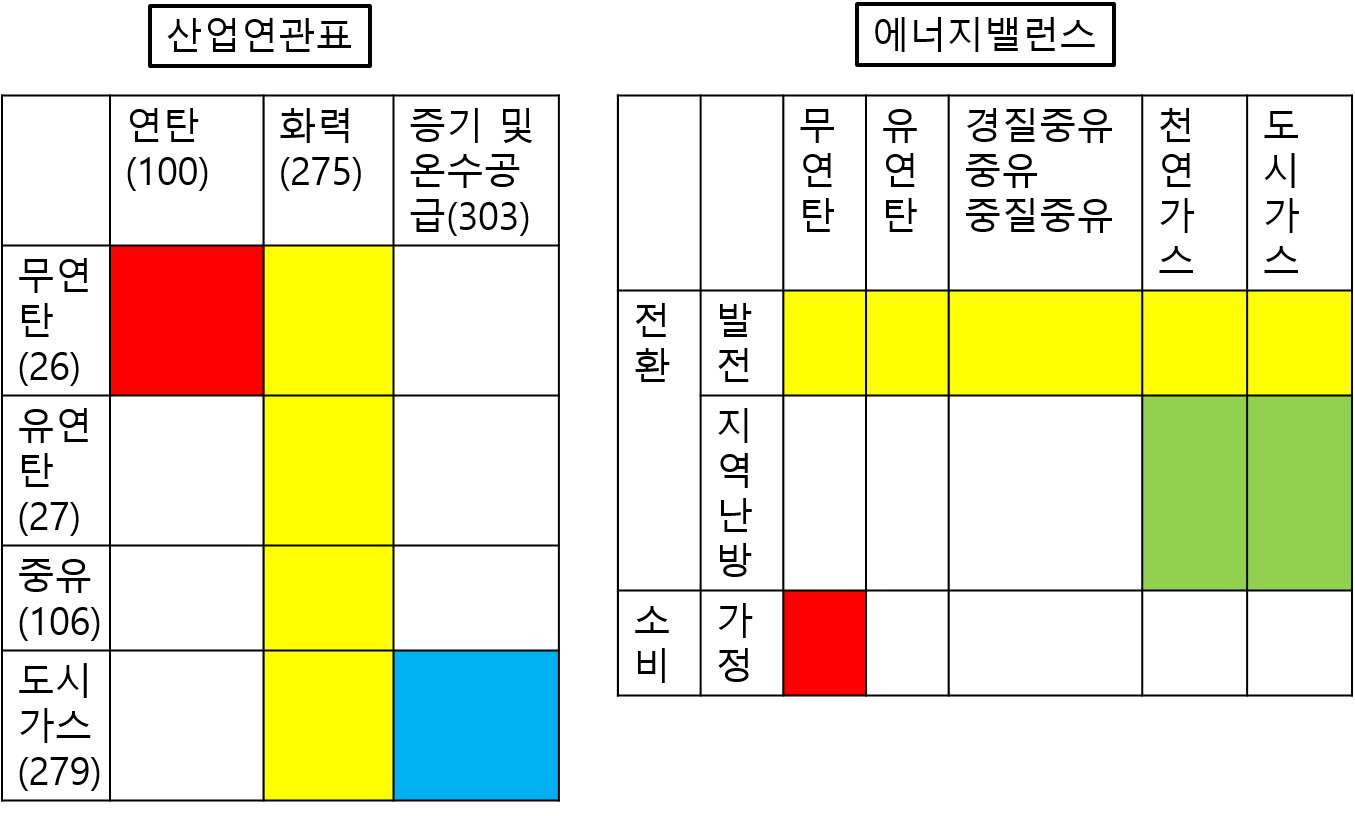
\includegraphics[width=1.00\textwidth]{Espec.png}
	%\caption{}
	%\label{IEA world balance}
	\end{figure}	
	
\end{frame}
%----------------------------------------------------------------------------------------------


%------------------------------- 슬라이드  --------------------------------------------------
\begin{frame}
	\frametitle{Step 3: 에너지 '총수요'를 산업연관표에 할당-(3) 나프타   }
\bigskip
\begin{small}
\begin{itemize}
\item{석유화학제품(111-138)에 투입된 나프타(101): 에너지 밸런스에서 석유화학산업 최종에너지소비에 할당된 나프타 에너지양을 석유화학제품 별 나프타 수요의 비중에 따라 우선할당}
\item{나머지 나프타 수요: 석유화학제품 이외의 산업에 투입된 양에 따라 할당}
\end{itemize}
\smallskip

\begin{eqnarray*}
E_{ij|j\in J}&=&\overline{E}(\mbox{정유 및 석유화학산업 나프타 최종에너지소비})\times\frac{IO_{i,j\in J}}{\Sigma_{j\in J}IO_{i,j}}\\
E_{ij|j \notin J}&=&(\mbox{에너지 총수요}(E_i)-\sum_{j\in J}E_{ij})\\
& &\times\frac{IO_{ij| j \notin J}}{\Sigma_{j}IO_{ij}+Household_i-\sum_{j\in J}IO_{ij}}\\
E_{i,h}&=&(\mbox{에너지 총수요}(E_i)-\sum_{j\in J}E_{ij})\\
& &\times\frac{Household_h}{\Sigma_{j}IO_{ij}+Household_i-\sum_{j\in J}IO_{ij}}
\end{eqnarray*}
\end{small}


%\begin{itemize}
%\item{input : E.Demand\_IO, IO\_whole}
%\item{process : ghg.r line 331-410}
%\item{output :Energy\_BE\_residual,Energy\_BE  }
%\end{itemize} 
\end{frame}
%----------------------------------------------------------------------------------------------

%------------------------------- 슬라이드  --------------------------------------------------
\begin{frame}
	\frametitle{Step 3: 에너지 '총수요'를 산업연관표에 할당-(4) 화력 및 자가발전 }
\bigskip
\begin{small}
\begin{itemize}
\item{화력에 우선 할당한 무연탄, 유연탄, 중유, 도시가스, 천연가 에너지를 제외한 나머지 에너지 분할}
\item{화력 및 자가발전 중간수요/가계수요 항목이 화력 총수요 + 자가발전 총수요에서 차지하는 비중에 따라 분할}
\end{itemize} 

\begin{eqnarray*}
E_{275,j|j\in J}&=&\overline{E}(\mbox{화력 투입 무연탄, 유연탄, 중유,도시가스, 천연가스 })\\
E_{ij|i\in(275,277),j \notin J}&=&(E_{275}+E_{277}-\sum_{j\in J}E_{275,j})\\
& &\times\frac{IO_{ij|i \in (275,277), j \notin J}}{\Sigma_{j}IO_{275,j}+\Sigma_{i\in(275,277)}Household_i-\sum_{j\in J}IO_{275,j}}\\
E_{i,h|i\in(275,277),j \notin J}&=&(E_{275}+E_{277}-\sum_{j\in J}E_{275,j})\\
& &\times\frac{Household_{i|i \in (275,277), j \notin J}}{\Sigma_{j}IO_{275,j}+\Sigma_{i\in(275,277)}Household_i-\sum_{j\in J}IO_{275,j}}\\
\end{eqnarray*}


%\begin{itemize}
%\item{input : E.Demand\_IO, IO\_whole}
%\item{process : ghg.r line 331-410}
%\item{output :Energy\_BE\_residual,Energy\_BE  }
%\end{itemize} 
\end{small}

\end{frame}
%----------------------------------------------------------------------------------------------



%*******************************
\section{Step 4:온실가스 계산 = 배출계수$\times$할당 에너지  }
%*******************************

%------------------------------- 슬라이드  --------------------------------------------------
\begin{frame}
	\frametitle{Step 4:온실가스 계산-(1) 기본공식}
\bigskip
\begin{enumerate}
\item{에너지 중간수요에 배출계수와 몰입률을 적용하여 온실가스 배출량 계산} 
\smallskip
\begin{displaymath}
			\mbox{온실가스 배출량} (G_{ij})=\left\{\begin{array}{lr}
\mbox{배출계수}(\theta_i)\times (1-Sunk_i)\times E_{ij}&\\
(\mbox{나프타, 윤활유})& \\
\mbox{배출계수}(\theta_i)\times E_{ij}&\\
(\mbox{for the rest})&\\
\end{array}\right.
\end{displaymath}
\begin{itemize}
\item{$Sunk_i$: 몰입률 = 연료가 아닌 중간재에 포함되는 탄소는 일부 제품에 체화(몰입)되므로 대기중의 온실가스로 전환되지 않음}
\end{itemize}
\bigskip
\item{제외항목= 수출, 고정자본형성, 재고, 이중계산}
\begin{itemize}
\item{소비과정에서 발생하는 온실가스만 계산: 수출, 고정자본형성, 재고조정에 할당된 에너지는 온실가스로 전환하지 않음}
\item{이중계산 방지: 전력 및 열에너지는 사용 시 온실가스가 배출되지 않는다고 가정}
\end{itemize}
\end{enumerate}
%\begin{small}
%\begin{itemize}
%\item{input : Energy\_BE,"EC1996.csv"}
%\item{process : ghg.r line 412-465}
%\item{output :ECO2}
%\end{itemize} 
%\end{small}	
\end{frame}
%----------------------------------------------------------------------------------------------


%-------------------------------- 슬라이드  -------------------------------------------------
\begin{frame}
	\frametitle{배출계수}
	  	\begin{figure}
	\centering
	 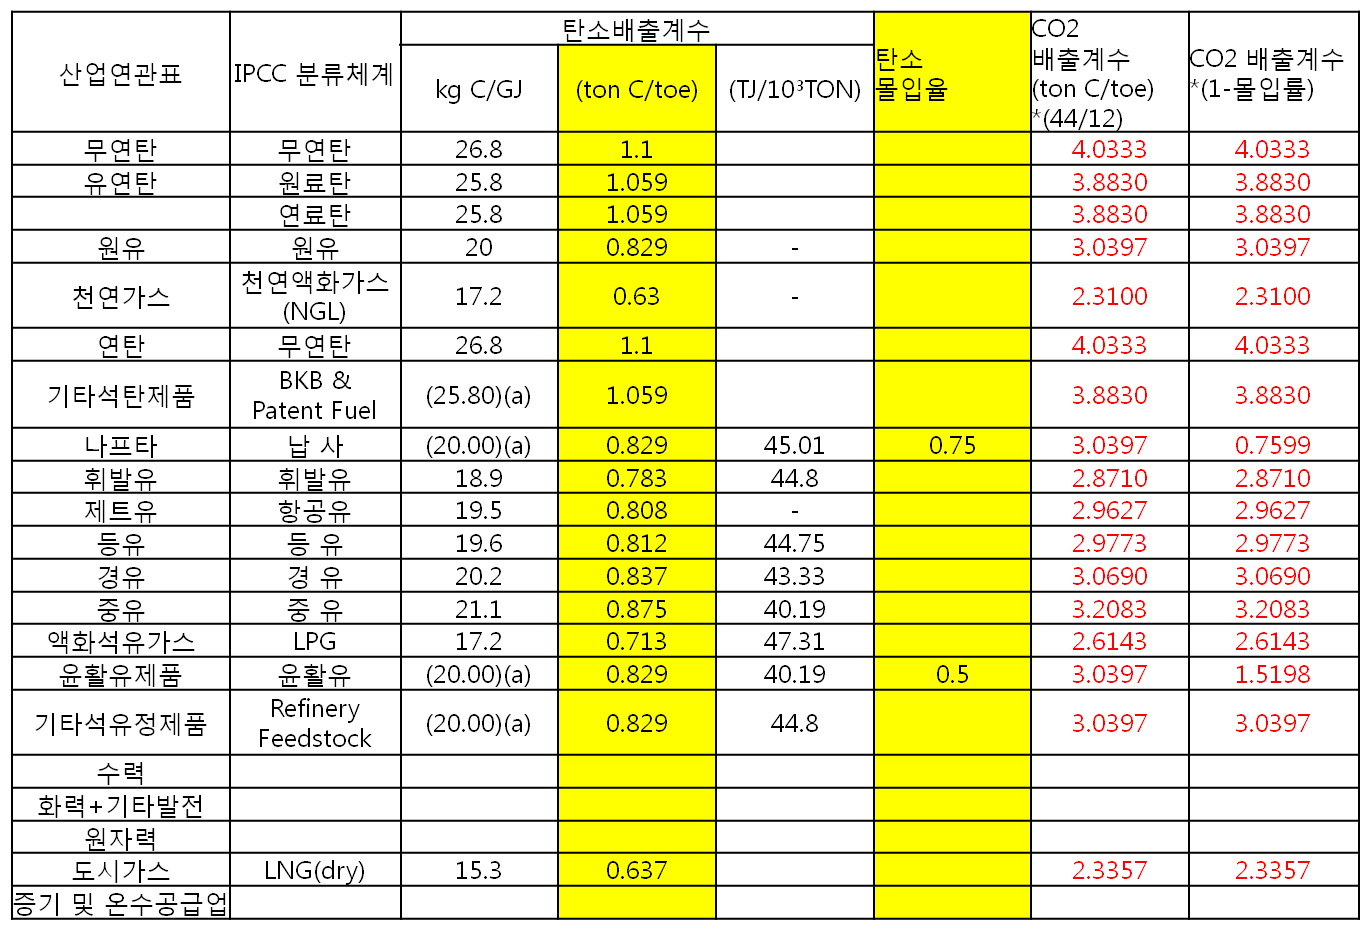
\includegraphics[width=1.00\textwidth]{ECform.png}
	%\caption{}
	%\label{IEA world balance}
	\end{figure}	
	
\end{frame}
%----------------------------------------------------------------------------------------------


%-------------------------------- 슬라이드  -------------------------------------------------
\begin{frame}
	\frametitle{제외항목: 수출, 고정자본형성, 재고, 이중계산 방지}
	  	\begin{figure}
	\centering
	 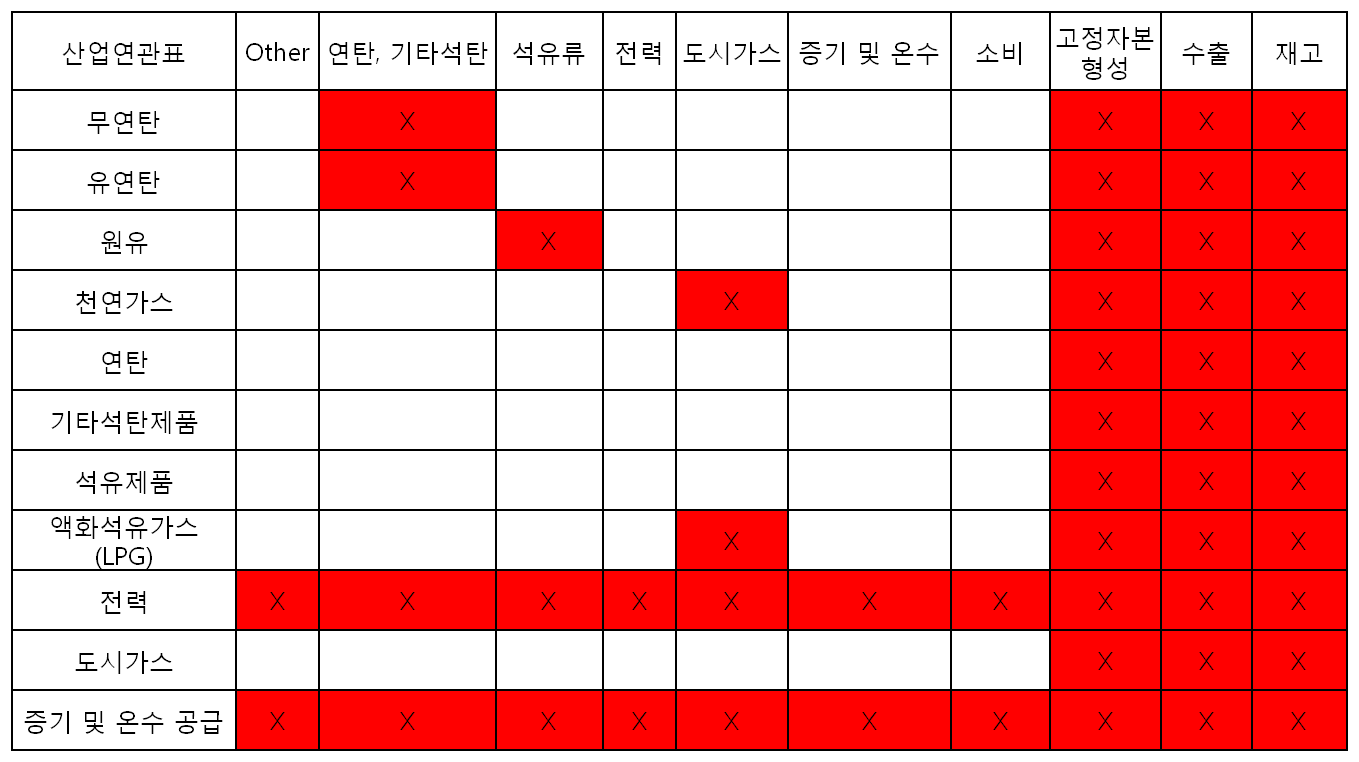
\includegraphics[width=1.00\textwidth]{noncount.png}
	%\caption{}
	%\label{IEA world balance}
	\end{figure}	
	
\end{frame}
%----------------------------------------------------------------------------------------------




%
%-------------------------------- 슬라이드  -------------------------------------------------
\begin{frame}
	\frametitle{}
	  	\begin{figure}
	\centering
	 
\includegraphics[width=1.00\textwidth]{thanks.png}
	%\caption{}
	%\label{IEA world balance}
	\end{figure}	
	
\end{frame}
%----------------------------------------------------------------------------------------------

\end{document}
%==========================  본문 끝 = ================================